\subsection{Validation-Selected Architecture Exploration}

\label{sec:architecture-search}

We extend the original decoder study with a separate, prospective architecture search. All historical default-model results above are retained. The search uses ETTh1 at $H=96$ and selects exclusively by validation pinball; test scores do not influence candidate ranking. Twelve prespecified candidates compare the original three-layer Transformer, no encoder, residual per-token MLPs, dilated temporal CNNs, a CNN--Transformer combination, a one-layer Transformer, and linear/MLP/CNN/patch direct heads. MLP and CNN residual blocks use pre-layer normalization, GELU, dropout, and a final layer normalization. CNN blocks use kernel size 3, dilations 1/2/4 and a pointwise output projection; the hybrid uses two CNN blocks followed by one Transformer block. The narrow CNN/MLP variants jointly change width to 64, FFN width to 128, and learning rate to $3\times10^{-4}$, so their comparison does not isolate those factors. The direct MLP maps the complete 336-step history through a 256-unit GELU hidden layer to $7H$ outputs. Every candidate retains training-only standardization and the ordered median/positive-gap output.

Screening uses seed 2024 and at most eight epochs. The three candidates with lowest screening validation loss, together with the original model, are retrained with seeds 2024/2025/2026 under the original 30-epoch policy. The minimum mean confirmation validation loss determines a frozen candidate; candidate identifiers break exact ties. This finite search does not establish global optimality, and short screening can miss slower-converging configurations. Repeated validation use also introduces selection optimism.

\begin{table*}[t]
\centering\small
\caption{Architecture selection on ETTh1 validation data at $H=96$. Screening is a single seed with eight epochs; confirmation entries require all three seeds and show mean $\pm$ sample SD. Dashes denote unconfirmed groups, not zero loss. Parameter counts are for $H=96$. No test score is used in this table.}
\label{tab:architecture-validation}
\begin{tabular}{@{}lrrr@{}}
\toprule
Candidate & Parameters & Screen val. & Confirm val. \\
\midrule
MLP-3, D64, lr 3e-4 & 142407 & 0.11941 & -- \\
CNN-direct & 3930144 & 0.12045 & -- \\
MLP-3 & 456775 & 0.12065 & -- \\
Patch-direct & 3932448 & 0.12108 & -- \\
MLP-direct & 258976 & 0.12124 & -- \\
CNN-3, D64, lr 3e-4 & 191559 & 0.12222 & -- \\
Transformer-1 & 390727 & 0.12372 & -- \\
CNN-3 & 653383 & 0.12395 & -- \\
Transformer-3 (original) & 655687 & 0.12481 & -- \\
No encoder & 257991 & 0.12492 & -- \\
Linear-NQ & 226464 & 0.12506 & -- \\
CNN + Transformer & 654151 & 0.12749 & -- \\
\bottomrule
\end{tabular}
\end{table*}


\begin{figure*}[t]\centering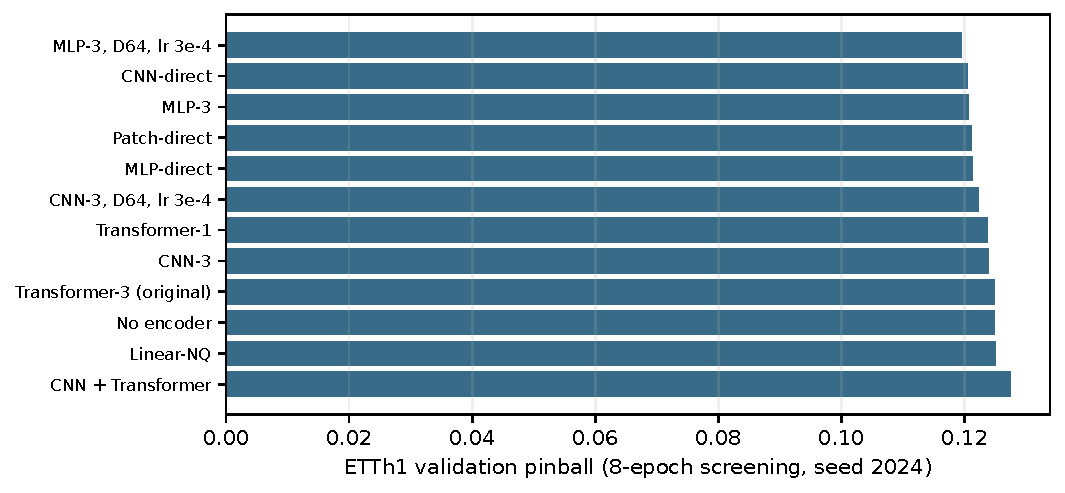
\includegraphics[width=.85\textwidth]{figures/architecture_screening.pdf}\caption{Completed eight-epoch validation screening runs. Bars rank validation loss; they are not test comparisons.}\Description{Horizontal bars compare completed architecture candidates on ETTh1 validation pinball.}\end{figure*}

At this export, 12 of 12 screening runs and 0 confirmation runs have completed. There are 0 completed full-test runs and 0 complete three-seed test groups in the extension.
